\documentclass[
11pt, % The default document font size, options: 10pt, 11pt, 12pt
%codirector, % Uncomment to add a codirector to the title page
]{charter} 
\renewcommand{\labelenumii}{\arabic{enumi}.\arabic{enumii}}
\renewcommand{\labelenumiii}{\arabic{enumi}.\arabic{enumii}.\arabic{enumiii}}
\renewcommand{\labelenumiv}{\arabic{enumi}.\arabic{enumii}.\arabic{enumiii}.\arabic{enumiv}}



% El títulos de la memoria, se usa en la carátula y se puede usar el cualquier lugar del documento con el comando \ttitle
\titulo{Sistema de monitoreo de ocupación en
espacios internos mediante BLE \textit{Beacons}} 

% Nombre del posgrado, se usa en la carátula y se puede usar el cualquier lugar del documento con el comando \degreename
%\posgrado{Carrera de Especialización en Sistemas Embebidos} 
\posgrado{Carrera de Especialización en Internet de las Cosas} 
%\posgrado{Carrera de Especialización en Intelegencia Artificial}
%\posgrado{Maestría en Sistemas Embebidos} 
%\posgrado{Maestría en Internet de las cosas}

% Tu nombre, se puede usar el cualquier lugar del documento con el comando \authorname
\autor{Ing. Facundo Fernández} 

% El nombre del director y co-director, se puede usar el cualquier lugar del documento con el comando \supname y \cosupname y \pertesupname y \pertecosupname
\director{Nombre del Director}
\pertenenciaDirector{pertenencia} 
% FIXME:NO IMPLEMENTADO EL CODIRECTOR ni su pertenencia
\codirector{John Doe} % para que aparezca en la portada se debe descomentar la opción codirector en el documentclass
\pertenenciaCoDirector{FIUBA}

% Nombre del cliente, quien va a aprobar los resultados del proyecto, se puede usar con el comando \clientename y \empclientename
\cliente{Nombre del cliente}
\empresaCliente{Empresa del cliente}

% Nombre y pertenencia de los jurados, se pueden usar el cualquier lugar del documento con el comando \jurunoname, \jurdosname y \jurtresname y \perteunoname, \pertedosname y \pertetresname.
\juradoUno{Nombre y Apellido (1)}
\pertenenciaJurUno{pertenencia (1)} 
\juradoDos{Nombre y Apellido (2)}
\pertenenciaJurDos{pertenencia (2)}
\juradoTres{Nombre y Apellido (3)}
\pertenenciaJurTres{pertenencia (3)}
 
\fechaINICIO{17 de octubre de 2023}		%Fecha de inicio de la cursada de GdP \fechaInicioName
\fechaFINALPlan{05 de diciembre de 2023} 	%Fecha de final de cursada de GdP
\fechaFINALTrabajo{16 de septiembre de 2024}	%Fecha de defensa pública del trabajo final


\begin{document}

\maketitle
\thispagestyle{empty}
\pagebreak


\thispagestyle{empty}
{\setlength{\parskip}{0pt}
\tableofcontents{}
}
\pagebreak


\section*{Registros de cambios}
\label{sec:registro}


\begin{table}[ht]
\label{tab:registro}
\centering
\begin{tabularx}{\linewidth}{@{}|c|X|c|@{}}
\hline
\rowcolor[HTML]{C0C0C0} 
Revisión & \multicolumn{1}{c|}{\cellcolor[HTML]{C0C0C0}Detalles de los cambios realizados} & Fecha      \\ \hline
0      & Creación del documento                                 &\fechaInicioName \\ \hline
1      & Se completa hasta el punto 5 inclusive                 & 31 de octubre de 2023 \\ \hline
2      & Se completa hasta el punto 9 inclusive & 7 de noviembre de 2023
%		  Se puede agregar algo más \newline
%		  En distintas líneas \newline
%		  Así                                                    & dd/mm/aaaa 
\\ \hline
%3      & Se completa hasta el punto 11 inclusive                & dd/mm/aaaa \\ \hline
%4      & Se completa el plan	                                 & dd/mm/aaaa \\ \hline
\end{tabularx}
\end{table}

\pagebreak



\section*{Acta de constitución del proyecto}
\label{sec:acta}

\begin{flushright}
Buenos Aires, \fechaInicioName
\end{flushright}

\vspace{2cm}

Por medio de la presente se acuerda con el Ing. \authorname\hspace{1px} que su Trabajo Final de la \degreename\hspace{1px} se titulará ``\ttitle'', consistirá esencialmente en la implementación de un prototipo de un sistema de monitoreo de ocupación utilizando \textit{Beacons Bluetooth Low Energy}, y tendrá un presupuesto preliminar estimado de {715} h de trabajo y {\$200} USD, con fecha de inicio \fechaInicioName\hspace{1px} y fecha de presentación pública \fechaFinalName.

Se adjunta a esta acta la planificación inicial.

\vfill

% Esta parte se construye sola con la información que hayan cargado en el preámbulo del documento y no debe modificarla
\begin{table}[ht]
\centering
\begin{tabular}{ccc}
\begin{tabular}[c]{@{}c@{}}Dr. Ing. Ariel Lutenberg \\ Director posgrado FIUBA\end{tabular} & \hspace{2cm} & \begin{tabular}[c]{@{}c@{}}\clientename \\ \empclientename \end{tabular} \vspace{2.5cm} \\ 
\multicolumn{3}{c}{\begin{tabular}[c]{@{}c@{}} \supname \\ Director del Trabajo Final\end{tabular}} \vspace{2.5cm} \\
%\begin{tabular}[c]{@{}c@{}}\jurunoname \\ Jurado del Trabajo Final\end{tabular}     &  & \begin{tabular}[c]{@{}c@{}}\jurdosname\\ Jurado del Trabajo Final\end{tabular}  \vspace{2.5cm}  \\
%\multicolumn{3}{c}{\begin{tabular}[c]{@{}c@{}} \jurtresname\\ Jurado del Trabajo Final\end{tabular}} \vspace{.5cm}                                                                     
\end{tabular}
\end{table}




\section{1. Descripción técnica-conceptual del proyecto a realizar}
\label{sec:descripcion}

El proyecto nace como un emprendimiento personal con un enfoque específico para gimnasios y recintos deportivos en donde los usuarios (clientes del gimnasio) pueden acceder a distintas horas sin ningún tipo de limitación. Este emprendimiento surge de la necesidad de entender el comportamiento de usuarios en gimnasios con el objetivo de proporcionar al cliente (propietario del gimnasio) la capacidad de entender a su clientela y cómo usan sus instalaciones. 

Adicional, esta herramienta permite entender el tiempo de visita de una persona. El tiempo de visita es una medida sumamente importante para entender a los usuarios que se mantienen como clientes de un gimnasio y a los que no. En el contexto de clientes de gimnasios, es más económico retener a una persona para que siga siendo cliente que conseguir nuevos. El objetivo general es poder dar una herramienta más a los gimnasios donde puedan utilizar datos para tomar decisiones de negocio.

Debido a que este proyecto es un prototipo y un emprendimiento personal, no se cuenta con financiamiento de ningún tipo, por lo que se trabajará en diseñar un sistema funcional que cumpla con las características de un mínimo producto viable, financiado completamente por el autor de este documento. Una de las ventajas de abordarlo de esta manera es que no existen limitaciones de desarrollo ni hay ningún interesado que pueda tener incidencia en el resultado final del trabajo.

En el contexto actual de la tecnología y la creciente demanda de soluciones de posicionamiento en interiores, el presente proyecto se centra en la implementación de un sistema innovador de monitoreo de ocupación en espacios interiores utilizando la tecnología \textit{Bluetooth Low Energy} (BLE) \textit{Beacons}. Esta tecnología permite la ubicación precisa de dispositivos móviles en entornos cerrados, brindando a los usuarios una experiencia de ubicación confiable y en tiempo real. 

La esencia de este proyecto radica en proporcionar a los propietarios de recintos o edificios una herramienta para la gestión eficiente de la ocupación, así como una herramienta más de recaudación de datos de uso y comportamiento. La solución propuesta se distingue por su capacidad para ofrecer datos precisos y actualizados sobre la cantidad de personas presentes en el recinto en cualquier momento dado, así como la capacidad de determinar el tiempo de visita promedio de un usuario.

El desafío que aborda este proyecto es la falta de sistemas de monitoreo de ocupación precisos y en tiempo real en entornos interiores. La tecnología BLE \textit{Beacons} junto con la estación base ESP32-C3 proporciona una solución efectiva y rentable. Mediante la emisión de señales de baja energía, los \textit{Beacons} identifican la presencia de dispositivos móviles, permitiendo a la aplicación de monitoreo determinar la ocupación actual a través de un algoritmo de triangulación. Esta información se almacena en una base de datos no relacional alojada en MongoDB, brindando al propietario acceso a datos cruciales para la toma de decisiones informadas.

El sistema se compone de cuatro elementos principales: los BLE \textit{Beacons}, la estación base ESP32-C3, la aplicación de monitoreo y la base de datos no relacional. Los \textit{Beacons} emiten señales identificativas, que son escaneadas por la estación base. La aplicación de monitoreo procesa estas señales para determinar la proximidad de los dispositivos móviles y actualiza la base de datos con la información de ocupación. A través de un panel de control intuitivo, el propietario del recinto puede visualizar la ocupación actual y acceder a informes históricos. En la figura \ref{fig:diagBloques} se presenta el diagrama de bloques del sistema, donde se observa claramente la distribución y diseño de los componentes clave.

\begin{figure}[htpb]
\centering 
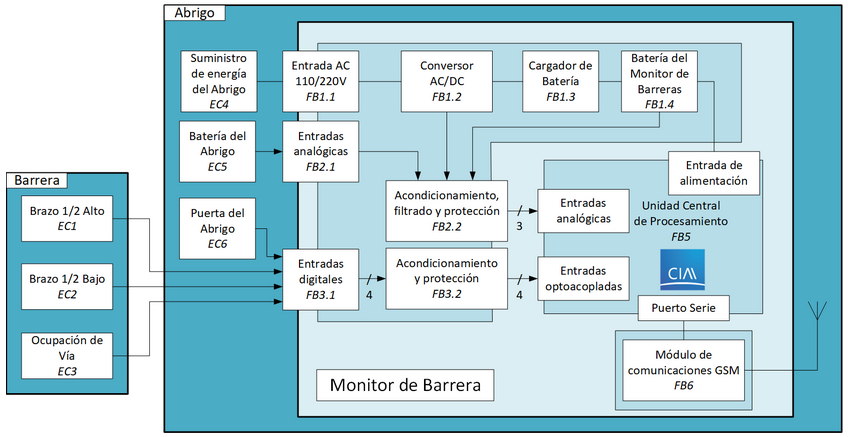
\includegraphics[width=.7\textwidth]{./Figuras/diagBloques.png}
\caption{Diagrama en bloques del sistema.}
\label{fig:diagBloques}
\end{figure}

\vspace{25px}

La innovación radica en la combinación efectiva de la tecnología BLE \textit{Beacons} con la estación base ESP32-C3 para ofrecer una solución escalable y rentable de monitoreo de ocupación en interiores. Esta solución se destaca por su capacidad para proporcionar datos precisos y accesibles, sentando las bases para futuras implementaciones en diversos entornos comerciales y públicos. 

Para la realización de este trabajo, se probarán y utilizarán hasta 6 \textit{beacons} o balizas en un entorno reducido, con el objetivo de probar la viabilidad del proyecto. Este entorno reducido no superará los 50 m$^2$ y será en un ambiente doméstico. Para el panel de control se creará una aplicación accesible sólo a través de web, con el objetivo de reducir costos de desarrollo.

\section{2. Identificación y análisis de los interesados}
\label{sec:interesados}

Dado que este proyecto es de carácter personal, no involucra a interesados externos o a un equipo de trabajo formal. En este contexto, la principal parte interesada es el autor, como el iniciador y ejecutor del proyecto. Como único responsable, el autor asume todas las funciones, desde la planificación y desarrollo hasta la gestión económica y control de entregables. Esta autonomía proporciona flexibilidad y agilidad en la toma de decisiones, permitiendo una ejecución eficiente del proyecto.

En calidad de responsable, el rol abarca la supervisión integral del proyecto, incluyendo la gestión económica, planificación de tareas, desarrollo de los componentes técnicos y aseguramiento de la calidad de los entregables. Además, el responsable asume la responsabilidad de mantener el proyecto dentro de los plazos establecidos y gestionar eficazmente los recursos disponibles.

El director, por su parte, desempeñará un papel esencial al brindar orientación y asesoramiento experto en todas las facetas del proyecto. Se espera que actúe como un referente en cuestiones técnicas y organizativas desde el inicio hasta la finalización del proyecto, aportando valiosos conocimientos y experiencia para asegurar su éxito. Su apoyo será fundamental para superar cualquier desafío que pueda surgir a lo largo del desarrollo del proyecto.

\begin{table}[ht]
%\caption{Identificación de los interesados}
%\label{tab:interesados}
\begin{tabularx}{\linewidth}{@{}|l|X|X|l|@{}}
\hline
\rowcolor[HTML]{C0C0C0} 
Rol           & Nombre y Apellido & Organización 	& Puesto 	\\ \hline
Cliente       & \clientename      &\empclientename	&        	\\ \hline
Responsable   & \authorname       & FIUBA        	& Alumno 	\\ \hline
Orientador    & \supname	      & \pertesupname 	& Director Trabajo final \\ \hline
\end{tabularx}
\end{table}



\section{3. Propósito del proyecto}
\label{sec:proposito}

El propósito de este proyecto es implementar un sistema de monitoreo de ocupación en espacios interiores, principalmente en gimnasios, mediante la tecnología \textit{Bluetooth Low Energy} (BLE) \textit{Beacons}. Se busca proporcionar al propietario del recinto datos precisos, históricos y de calidad sobre la cantidad de personas presentes en cualquier momento dado, permitiendo así una gestión eficiente de la ocupación y una toma de decisiones informadas a través de datos con el objetivo de medir el comportamiento de los usuarios. Esta solución pionera sienta las bases para futuras implementaciones en diversos entornos comerciales y públicos, abriendo nuevas posibilidades en el campo del posicionamiento en interiores.

\section{4. Alcance del proyecto}
\label{sec:alcance}

El presente proyecto incluye:
\begin{itemize}
	\item La planificación, diseño, implementación y puesta en funcionamiento de un sistema de monitoreo de ocupación en espacios interiores utilizando la tecnología \textit{Bluetooth Low Energy} (BLE) \textit{Beacons} en un espacio no mayor a los 50 m$^2$.
	\item La adquisición y ubicación estratégica de los BLE \textit{Beacons}, así como la configuración de la estación base ESP32-C3 y el desarrollo de la aplicación web de monitoreo. 
	\item La implementación de una base de datos no relacional en MongoDB para el almacenamiento y gestión de la información de ocupación. 
	\item Pruebas para verificar el funcionamiento correcto del sistema 
	\item Una interfaz de usuario intuitiva en forma de panel de control para que el propietario del recinto pueda visualizar la ocupación actual, acceder a informes históricos y analizar los datos si lo considera necesario.
	\item La cobertura de todos los costos relacionados con el desarrollo, como son el hardware y software por parte del autor.
\end{itemize}


El presente proyecto no incluye:
\begin{itemize}
	\item La adquisición de hardware o software adicional no especificado en los requerimientos, salvo que sea necesario para la integración del sistema y se determine previamente.
	\item La adquisición o configuración de servicios de conectividad de red, como proveedores de internet o servicios de datos móviles.
	\item Mantenimiento continuo del sistema después de la finalización del proyecto.
	\item La capacitación avanzada en programación o configuración de hardware que no esté directamente relacionada con el sistema implementado.
	\item Una aplicación de configuración del sistema, a menos que el autor lo requiera.
\end{itemize}

Cualquier modificación o extensión del alcance del proyecto requerirá una revisión y aprobación previa por parte del director del proyecto y el responsable de este.


\section{5. Supuestos del proyecto}
\label{sec:supuestos}

\begin{itemize}
	\item Disponibilidad de recursos humanos: se asume que el responsable del proyecto contará con el tiempo y dedicación necesarios para llevar a cabo todas las etapas de planificación, implementación y puesta en marcha del sistema. Además, se presupone la colaboración activa del director para brindar orientación técnica y organizativa.
	\item Estabilidad de las condiciones del entorno: se supone que las condiciones ambientales y estructurales en los recintos seleccionados serán estables y no experimentarán cambios significativos durante el período de implementación del proyecto. Por condiciones ambientales y estructurales se refiere a la disposición física del espacio como paredes y muebles, así como fluctuaciones significativas en la temperatura o en la humedad ya que estas pueden influir en cómo las señales \textit{Bluetooth} se propagan en el espacio.
	\item Disponibilidad de equipamiento y materiales: se presupone que se podrá adquirir el hardware necesario, incluyendo los BLE \textit{Beacons} y la estación base ESP32-C3, así como cualquier otro equipo o material requerido para la implementación del sistema.
	\item Presupuesto: se supone que el presupuesto establecido de {\$200} USD será suficiente para cubrir los costos de hardware y software, así como cualquier otro material requerido para la implementación del sistema. En caso de incurrir en un gasto mayor, se evaluará la viabilidad, manteniendo un tope máximo de {\$1,000} USD.
	\item Factibilidad técnica: se considera que la tecnología BLE \textit{Beacons} y el microcontrolador ESP32-C3 son adecuados para la aplicación prevista y no presentarán inconvenientes técnicos significativos en su configuración y funcionamiento.
	\item Cumplimiento de regulaciones y normativas: se parte del supuesto de que el proyecto cumple con todas las regulaciones y normativas locales, estatales y federales aplicables y que no se requerirá de permisos o licencias adicionales para la implementación del sistema.
	\item Estabilidad de los protocolos de comunicación: se presupone que los protocolos de Internet estándar seleccionados (HTTP o MQTT) para la comunicación entre la aplicación móvil y la base de datos funcionarán de manera estable y confiable.
	\item Acceso a la tecnología y herramientas: se asume que se contará con acceso a las tecnologías y herramientas necesarias para el desarrollo de la aplicación de monitoreo y la configuración de la base de datos en MongoDB.
	\item Disponibilidad de energía eléctrica: se presupone que se dispondrá de suministro eléctrico confiable ya sea a través de baterías o red eléctrica para alimentar tanto los BLE \textit{Beacons} como la estación base y demás equipos asociados al sistema.
	\item Compatibilidad de dispositivos móviles: se supone que los dispositivos móviles que se encuentren en el rango de los BLE \textit{Beacons} serán compatibles con la tecnología \textit{Bluetooth Low Energy} y podrán recibir las señales emitidas. 
\end{itemize}

\section{6. Requerimientos}
\label{sec:requerimientos}

\begin{enumerate}
	\item Requerimientos funcionales
		\begin{enumerate}
			\item Funcionalidades
				\begin{enumerate}
					\item El sistema debe ser capaz de recibir señales BLE de hasta 6 \textit{beacons}.
					\item El sistema debe actualizarse en tiempo real o en un tiempo menor a dos minutos.
					\item El sistema debe poder determinar un identificador para cada dispositivo.
					\item El sistema debe ser capaz de procesar las señales y enviarlas a la base de datos en MongoDB.
					\item El sistema debe implementar un algoritmo de triangulación basado en las señales recibidas.
					\item El sistema debe poder determinar la ubicación de un dispositivo determinado.
					\item El sistema debe poder determinar la cantidad de tiempo que un dispositivo estuvo en un lugar.
					\item El sistema debe proporcionar una interfaz de usuario para visualizar y acceder a los datos.
				\end{enumerate}
			\item Configuración del sistema
				\begin{enumerate}
					\item El sistema debe ser capaz de gestionar la conexión y comunicación entre los \textit{beacons} (ESP32-C3 \textit{Bluetooth Low Energy}) y los dispositivos de procesamiento (\textit{Hub} - ESP32-C3).
					\item El sistema debe permitir la configuración de parámetros como la potencia de transmisión de los \textit{beacons} y la frecuencia de actualización de la ubicación.
				\end{enumerate}
			\item Protocolo MQTT
				\begin{enumerate}
					\item El protocolo utilizado para la gestión y envío de datos será MQTT.
					\item El sistema debe garantizar la fiabilidad y consistencia en el envío de datos a través del protocolo MQTT.
					\item Se deben establecer mecanismos de detección y gestión de errores en el envío de datos a través de MQTT, asegurando la resiliencia del sistema ante posibles fallos de comunicación.
					\item El sistema debe ser capaz de manejar la concurrencia de múltiples dispositivos enviando datos a través de MQTT de manera simultánea.
					\item Se debe proporcionar un mecanismo de notificación o alerta en caso de fallos en la comunicación a través de MQTT para permitir una respuesta rápida y eficaz.
				\end{enumerate}
		\end{enumerate}
	\item Requerimientos de documentación
		\begin{enumerate}
			\item Deberá proporcionarse documentación detallada sobre la configuración y conexión de los \textit{beacons} BLE (ESP32-C3).
			\item Se deberá documentar el proceso de configuración y programación del dispositivo de procesamiento (ESP32-C3) para actuar como \textit{hub}.
			\item Se debe generar documentación sobre el algoritmo de triangulación utilizado, incluyendo diagramas y fórmulas utilizadas.
			\item Se debe proporcionar una guía de usuario para la interfaz de usuario del panel de control.
			\item Documentación de código: comentarios detallados en el código fuente para facilitar el mantenimiento y comprensión futura.
			\item Deberá proporcionarse documentación detallada sobre la configuración de parámetros, como la potencia de transmisión de los \textit{beacons} y la frecuencia de actualización de la ubicación.
		\end{enumerate}
	\item Requerimiento de \textit{testing}
		\begin{enumerate}
			\item Se deben realizar pruebas de funcionamiento para garantizar que el sistema pueda determinar la ubicación del dispositivo con la precisión especificada.
			\item Pruebas de estrés para verificar el rendimiento del sistema bajo cargas máximas esperadas.
			\item Pruebas de seguridad para identificar y mitigar posibles vulnerabilidades en la comunicación entre el \textit{hub} y los \textit{beacons}.
			\item Pruebas de conectividad y comunicación entre los \textit{beacons} y el \textit{hub} para asegurar una transmisión de señal confiable.
		\end{enumerate}
	\item Requerimientos de la interfaz de usuario
		\begin{enumerate}
			\item La interfaz de usuario debe ser intuitiva y fácil de usar, permitiendo la visualización de la ubicación del dispositivo de manera clara y precisa.
			\item Debe haber opciones para filtrar y buscar registros de ubicaciones en la base de datos.
			\item La interfaz de usuario debe ser completamente responsiva y compatible con dispositivos móviles para facilitar su acceso desde diferentes plataformas.
			\item Se deben implementar mecanismos de notificación o alerta en caso de fallos en la determinación de la ubicación del dispositivo.
		\end{enumerate}
	\item Requerimientos interoperabilidad
		\begin{enumerate}
			\item El sistema debe ser compatible con diferentes versiones de \textit{beacons} BLE y dispositivos móviles con \textit{bluetooth}.
			\item Debe ser posible integrar el sistema con otras aplicaciones o sistemas a través de una API.
			\item El sistema debe ser compatible con diferentes sistemas operativos de dispositivos móviles, como iOS y Android.
		\end{enumerate}
	\item Requerimientos de seguridad y cumplimiento normativo
		\begin{enumerate}
			\item El sistema debe cumplir con las regulaciones y normas de privacidad de datos vigentes, como GDPR u otras aplicables.
			\item Debe implementarse un sistema de autenticación y autorización para acceder a la interfaz de usuario y los datos almacenados en MongoDB.
			\item Debe establecerse un registro de auditoría para rastrear el acceso y las acciones realizadas en la base de datos y la interfaz de usuario.
			\item Se debe implementar encriptación de extremo a extremo para proteger la comunicación entre los \textit{beacons}, el \textit{hub} y la base de datos.
		\end{enumerate}
\end{enumerate}

\section{7. Historias de usuarios (\textit{Product backlog})}
\label{sec:backlog}

El criterio de selección de los \textit{story points} utilizado fue el que se puede observar en la figura \ref{fig:storyCriteria}. Se evaluó la complejidad y la incertidumbre de cada historia de usuario, con un máximo de puntos de 21 por historia.

\begin{figure}[htpb]
\centering 
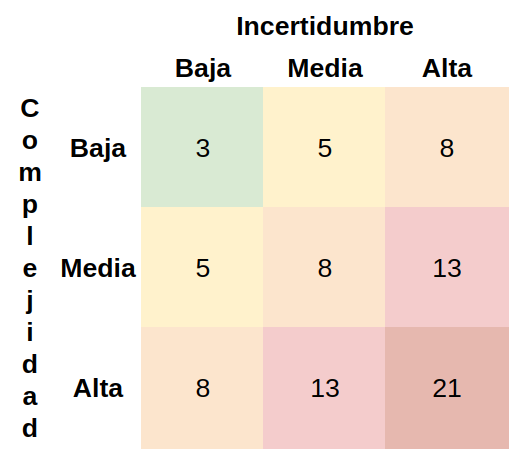
\includegraphics[width=.5\textwidth]{./Figuras/storyCriteria.png}
\caption{Criterio para el cálculo de los \textit{story points}.}
\label{fig:storyCriteria}
\end{figure}

\begin{enumerate}
	\item Como administrador del sistema, quiero recibir señales BLE de hasta 6 \textit{beacons} para obtener datos de ubicación precisos. \textit{Story points}: 13
	\item Como administrador del sistema, quiero que las actualizaciones se realicen en tiempo real o en un máximo de dos minutos para garantizar la frescura de los datos. \textit{Story points}: 5
	\item Como administrador del sistema, quiero que cada dispositivo tenga un identificador único para poder rastrearlos de manera individual. \textit{Story points}: 5
	\item Como administrador del sistema, quiero que el sistema procese y envíe las señales a la base de datos en MongoDB para almacenar la información. \textit{Story points}: 8
	\item Como administrador del sistema, quiero que se implemente un algoritmo de triangulación basado en las señales recibidas para determinar la ubicación de los dispositivos. \textit{Story points}: 13
	\item Como administrador del sistema, quiero poder determinar la ubicación de un dispositivo específico para responder a solicitudes de localización. \textit{Story points}: 8
	\item Como administrador del sistema, quiero poder determinar cuánto tiempo un dispositivo estuvo en un lugar para analizar patrones de movimiento. \textit{Story points}: 8
	\item Como administrador del sistema, quiero proporcionar una interfaz de usuario intuitiva y accesible para que los usuarios puedan visualizar y acceder a los datos de ubicación. \textit{Story points}: 13
	\item Como administrador del sistema, quiero gestionar la conexión y comunicación entre los \textit{beacons} y los dispositivos de procesamiento para asegurar una transmisión confiable. \textit{Story points}: 8
	\item Como administrador del sistema, quiero permitir la configuración de parámetros como la potencia de transmisión de los \textit{beacons} y la frecuencia de actualización de la ubicación para adaptar el sistema a diferentes entornos. \textit{Story points}: 5
	\item Como administrador del sistema, quiero utilizar el protocolo MQTT para la gestión y envío de datos para asegurar una comunicación eficiente. \textit{Story points}: 5
	\item Como administrador del sistema, quiero garantizar la fiabilidad y consistencia en el envío de datos a través del protocolo MQTT para evitar pérdida de información. \textit{Story points}: 8
	\item Como administrador del sistema, quiero establecer mecanismos de detección y gestión de errores en el envío de datos a través de MQTT para asegurar la resiliencia del sistema. \textit{Story points}: 8
	\item Como administrador del sistema, quiero manejar la concurrencia de múltiples dispositivos enviando datos a través de MQTT simultáneamente para garantizar un rendimiento óptimo. \textit{Story points}: 8
	\item Como administrador del sistema, quiero recibir notificaciones en caso de fallos en la comunicación a través de MQTT para responder de manera efectiva. \textit{Story points}: 5
	\item Como administrador del sistema, quiero proporcionar documentación detallada sobre la configuración y conexión de los \textit{beacons} BLE (ESP32-C3) para facilitar la instalación y configuración. \textit{Story points}: 5
	\item Como administrador del sistema, quiero documentar el proceso de configuración y programación del dispositivo de procesamiento (ESP32-C3) para actuar como \textit{hub} para ayudar a los usuarios en el proceso de configuración. \textit{Story points}: 5
	\item Como administrador del sistema, quiero generar documentación sobre el algoritmo de triangulación utilizado, incluyendo diagramas y fórmulas utilizadas para proporcionar información detallada sobre el funcionamiento del sistema. \textit{Story points}: 8
	\item Como administrador del sistema, quiero proporcionar una guía de usuario para la interfaz de usuario del panel de control para facilitar su uso. \textit{Story points}: 5
	\item Como administrador del sistema, quiero incluir comentarios detallados en el código fuente para facilitar el mantenimiento y comprensión futura del sistema. \textit{Story points}: 5
	\item Como administrador del sistema, quiero proporcionar documentación detallada sobre la configuración de parámetros, como la potencia de transmisión de los \textit{beacons} y la frecuencia de actualización de la ubicación, para que los usuarios puedan personalizar la configuración según sus necesidades. \textit{Story points}: 5
	\item Como administrador del sistema, quiero realizar pruebas de funcionamiento para garantizar que el sistema pueda determinar la ubicación del dispositivo con la precisión especificada. \textit{Story points}: 8
	\item Como administrador del sistema, quiero realizar pruebas de estrés para verificar el rendimiento del sistema bajo cargas máximas esperadas para asegurar su escalabilidad. \textit{Story points}: 8
	\item Como administrador del sistema, quiero realizar pruebas de seguridad para identificar y mitigar posibles vulnerabilidades en la comunicación entre el hub y los \textit{beacons} para garantizar la seguridad de los datos. \textit{Story points}: 8
	\item Como administrador del sistema, quiero realizar pruebas de conectividad y comunicación entre los \textit{beacons} y el \textit{hub} para asegurar una transmisión de señal confiable. \textit{Story points}: 8
	\item Como administrador del sistema, quiero que la interfaz de usuario sea intuitiva y fácil de usar, permitiendo la visualización de la ubicación del dispositivo de manera clara y precisa. \textit{Story points}: 8
	\item Como administrador del sistema, quiero opciones para filtrar y buscar registros de ubicaciones en la base de datos para facilitar la navegación y búsqueda de información. \textit{Story points}: 5
	\item Como administrador del sistema, quiero que la interfaz de usuario sea completamente responsiva y compatible con dispositivos móviles para garantizar la accesibilidad desde diferentes plataformas. \textit{Story points}: 5
	\item Como administrador del sistema, quiero implementar mecanismos de notificación o alerta en caso de fallos en la determinación de la ubicación del dispositivo para poder responder de manera proactiva. \textit{Story points}: 5
	\item Como administrador del sistema, quiero que el sistema sea compatible con diferentes versiones de \textit{beacons} BLE y dispositivos móviles con Bluetooth para garantizar la flexibilidad y compatibilidad. \textit{Story points}: 8
	\item Como administrador del sistema, quiero que el sistema sea capaz de integrarse con otras aplicaciones o sistemas a través de una API para permitir la expansión y personalización del sistema. \textit{Story points}: 8
	\item Como administrador del sistema, quiero que el sistema sea compatible con diferentes sistemas operativos de dispositivos móviles, como iOS y Android, para asegurar una amplia cobertura de usuarios. \textit{Story points}: 8
	\item Como administrador del sistema, quiero garantizar que el sistema cumple con las regulaciones y normas de privacidad de datos vigentes, como GDPR u otras aplicables, para garantizar la protección de la privacidad del usuario. \textit{Story points}: 8
	\item Como administrador del sistema, quiero implementar un sistema de autenticación y autorización para acceder a la interfaz de usuario y los datos almacenados en MongoDB para proteger la seguridad de la información. \textit{Story points}: 8
	\item Como administrador del sistema, quiero establecer un registro de auditoría para rastrear el acceso y las acciones realizadas en la base de datos y la interfaz de usuario para garantizar la trazabilidad de las operaciones. \textit{Story points}: 8
	\item Como administrador del sistema, quiero implementar encriptación de extremo a extremo para proteger la comunicación entre los \textit{beacons}, el \textit{hub} y la base de datos para garantizar la integridad y seguridad de los datos. \textit{Story points}: 8
	\item Como administrador del sistema, quiero implementar medidas de seguridad adicionales para proteger la integridad y privacidad de los datos transmitidos a través del protocolo MQTT. \textit{Story points}: 8
\end{enumerate}

\section{8. Entregables principales del proyecto}
\label{sec:entregables}

Los entregables del proyecto son los siguientes:

\begin{itemize}
	\item Documentación sobre la configuración y programación del dispositivo de procesamiento (ESP32-C3) para actuar como \textit{hub}.
	\item Documentación del algoritmo de triangulación utilizado, incluyendo diagramas y fórmulas.
	\item Guía de usuario para la interfaz de usuario del panel de control.
	\item Documentación de código con comentarios detallados.
	\item Diagrama de circuitos esquemáticos de la configuración hardware.
	\item Código fuente del firmware para los \textit{beacons} y el dispositivo de procesamiento.
	\item Diagrama de instalación que ilustre la disposición de los \textit{beacons} y el dispositivo de procesamiento.
	\item Informe final que incluya una descripción detallada del proyecto, sus objetivos, requisitos, implementación y resultados.
	\item Pruebas de funcionamiento documentadas, incluyendo resultados y conclusiones.
	\item Resultados de pruebas con análisis y recomendaciones.
	\item Informe de pruebas de seguridad con posibles vulnerabilidades identificadas y soluciones propuestas.
	\item Documentación sobre la configuración de parámetros, como la potencia de transmisión de los beacons y la frecuencia de actualización de la ubicación.
	\item Diagrama de flujo del proceso de comunicación entre los \textit{beacons}, el \textit{hub} y la base de datos.
	\item Prototipos y muestras físicas de los \textit{beacons} y el resto del hardware (si aplica).
	\item Presentación ejecutiva del proyecto para resumir los logros y beneficios del sistema.
	\item Archivos de configuración y \textit{scripts} de despliegue para facilitar la implementación en un entorno de producción.

\end{itemize}

\section{9. Desglose del trabajo en tareas}
\label{sec:wbs}

\begin{enumerate}
\item Grupo de Tareas 1: gestión y planificación del proyecto (50 h)
	\begin{enumerate}
	\item Planificación y programación del proyecto (30 h)
	\item Corrección de plan de proyecto (10 h)
	\item Gestión del tiempo del proyecto (10 h)
	\end{enumerate}
\item Grupo de Tareas 2: investigación y planificación inicial (55 h)
	\begin{enumerate}
	\item Investigación sobre tecnología BLE y \textit{beacons} (20 h)
	\item Análisis de requisitos y definición de alcance (15 h)
	\item Diseño preliminar de la arquitectura del sistema (20 h)
	\end{enumerate}
\item Grupo de Tareas 3: configuración de \textit{beacons} y dispositivos ESP32-C3 (105 h)
	\begin{enumerate}
	\item Investigación y documentación sobre la configuración de \textit{beacons} BLE (25 hs)
	\item Programación y configuración de los \textit{beacons} BLE (30 h)
	\item Configuración de dispositivos ESP32-C3 como \textit{hubs} (30 h)
	\item Pruebas de conectividad entre \textit{beacons} y \textit{hubs} (20 h)
	\end{enumerate}
\item Grupo de Tareas 4: desarrollo de algoritmo de triangulación (70 h)
	\begin{enumerate}
	\item Investigación y selección de algoritmo de triangulación (30 h)
	\item Implementación y pruebas del algoritmo de triangulación (40 h)
	\end{enumerate}
\item Grupo de Tareas 5: desarrollo de comunicación con MongoDB y MQTT (80 h)
	\begin{enumerate}
	\item Configuración y conexión con la base de datos MongoDB (25 h)
	\item Implementación del protocolo MQTT para comunicación (35 h)
	\item Pruebas de envío de datos a la base de datos (20 h)
	\end{enumerate}
\item Grupo de Tareas 6: desarrollo de interfaz de usuario (panel de control) (90 h)
	\begin{enumerate}
	\item Diseño y maquetación de la interfaz de usuario (30 h)
	\item Desarrollo de la interfaz de usuario (40 h)
	\item Implementación de filtros y opciones de búsqueda (20 h)
	\end{enumerate}
\item Grupo de Tareas 7: documentación y pruebas (155 h)
	\begin{enumerate}
	\item Documentación detallada de configuración de \textit{beacons} BLE (20 h)
	\item Documentación de configuración de dispositivos ESP32-C3 como \textit{hubs} (20 h)
	\item Documentación del algoritmo de triangulación (25 h)
	\item Pruebas de funcionamiento y precisión de la ubicación (30 h)
	\item Pruebas de estrés y rendimiento del sistema (30 h)
	\item Pruebas de seguridad y mitigación de vulnerabilidades (30 h)
	\end{enumerate}
\item Grupo de Tareas 8: seguridad y cumplimiento normativo (50 h)
	\begin{enumerate}
	\item Implementación de medidas de seguridad (25 h)
	\item Cumplimiento normativo y preparación de documentación (25 h)
	\end{enumerate}
\item Grupo de Tareas 9: tareas de cierre (60 h)
	\begin{enumerate}
	\item Generación de manuales y documentación final (25 h)
	\item Preparación de la presentación ejecutiva (15 h)
	\item Validación y pruebas finales antes de la entrega (20 h)
	\end{enumerate}
\end{enumerate}

Cantidad total: 715 horas.

\section{10. Diagrama de Activity On Node}
\label{sec:AoN}

\begin{consigna}{red}
Armar el AoN a partir del WBS definido en la etapa anterior. 

%La figura \ref{fig:AoN} fue elaborada con el paquete latex tikz y pueden consultar la siguiente referencia \textit{online}:

%\url{https://www.overleaf.com/learn/latex/LaTeX_Graphics_using_TikZ:_A_Tutorial_for_Beginners_(Part_3)\%E2\%80\%94Creating_Flowcharts}

\end{consigna}

\begin{figure}[htpb]
\centering 
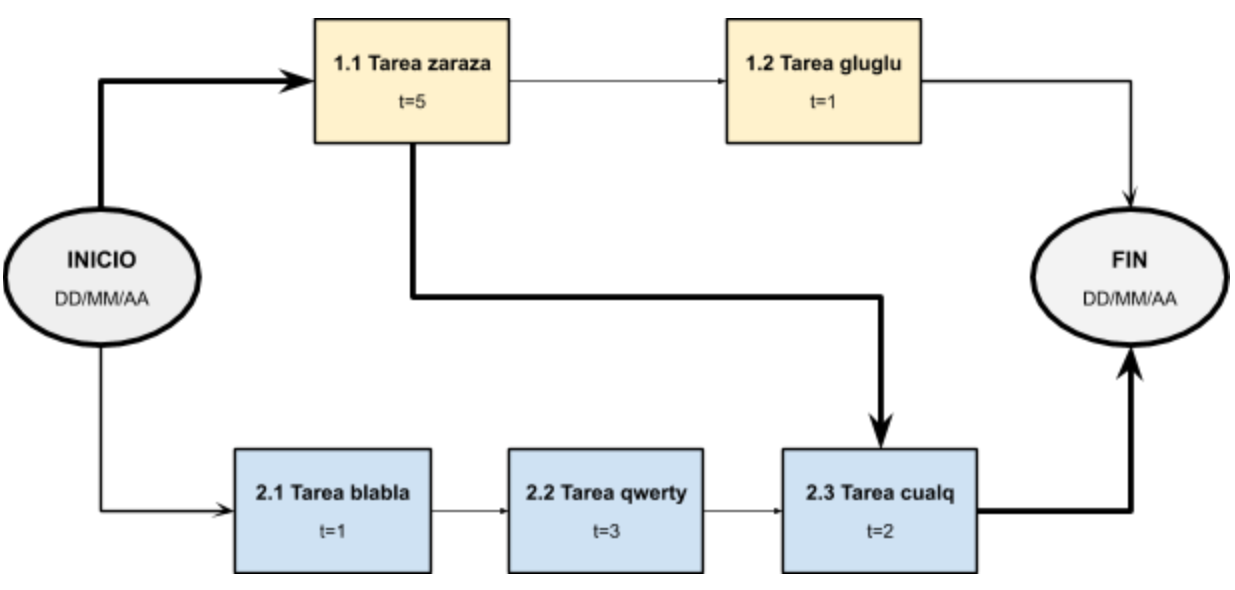
\includegraphics[width=.8\textwidth]{./Figuras/AoN.png}
\caption{Diagrama de \textit{Activity on Node}.}
\label{fig:AoN}
\end{figure}

Indicar claramente en qué unidades están expresados los tiempos.
De ser necesario indicar los caminos semicríticos y analizar sus tiempos mediante un cuadro.
Es recomendable usar colores y un cuadro indicativo describiendo qué representa cada color, como se muestra en el siguiente ejemplo:



\section{11. Diagrama de Gantt}
\label{sec:gantt}

\begin{consigna}{red}

Existen muchos programas y recursos \textit{online} para hacer diagramas de Gantt, entre los cuales destacamos:

\begin{itemize}
\item Planner
\item GanttProject
\item Trello + \textit{plugins}. En el siguiente link hay un tutorial oficial: \\ \url{https://blog.trello.com/es/diagrama-de-gantt-de-un-proyecto}
\item Creately, herramienta online colaborativa. \\\url{https://creately.com/diagram/example/ieb3p3ml/LaTeX}
\item Se puede hacer en latex con el paquete \textit{pgfgantt}\\ \url{http://ctan.dcc.uchile.cl/graphics/pgf/contrib/pgfgantt/pgfgantt.pdf}
\end{itemize}

Pegar acá una captura de pantalla del diagrama de Gantt, cuidando que la letra sea suficientemente grande como para ser legible. 
Si el diagrama queda demasiado ancho, se puede pegar primero la ``tabla'' del Gantt y luego pegar la parte del diagrama de barras del diagrama de Gantt.

Configurar el software para que en la parte de la tabla muestre los códigos del EDT (WBS).\\
Configurar el software para que al lado de cada barra muestre el nombre de cada tarea.\\
Revisar que la fecha de finalización coincida con lo indicado en el Acta Constitutiva.

En la figura \ref{fig:gantt}, se muestra un ejemplo de diagrama de Gantt realizado con el paquete de \textit{pgfgantt}. En la plantilla pueden ver el código que lo genera y usarlo de base para construir el propio.

\begin{figure}[htbp]
\begin{center}
\begin{ganttchart}{1}{12}
  \gantttitle{2020}{12} \\
  \gantttitlelist{1,...,12}{1} \\
  \ganttgroup{Group 1}{1}{7} \\
  \ganttbar{Task 1}{1}{2} \\
  \ganttlinkedbar{Task 2}{3}{7} \ganttnewline
  \ganttmilestone{Milestone o hito}{7} \ganttnewline
  \ganttbar{Final Task}{8}{12}
  \ganttlink{elem2}{elem3}
  \ganttlink{elem3}{elem4}
\end{ganttchart}
\end{center}
\caption{Diagrama de Gantt de ejemplo}
\label{fig:gantt}
\end{figure}


\begin{landscape}
\begin{figure}[htpb]
\centering 
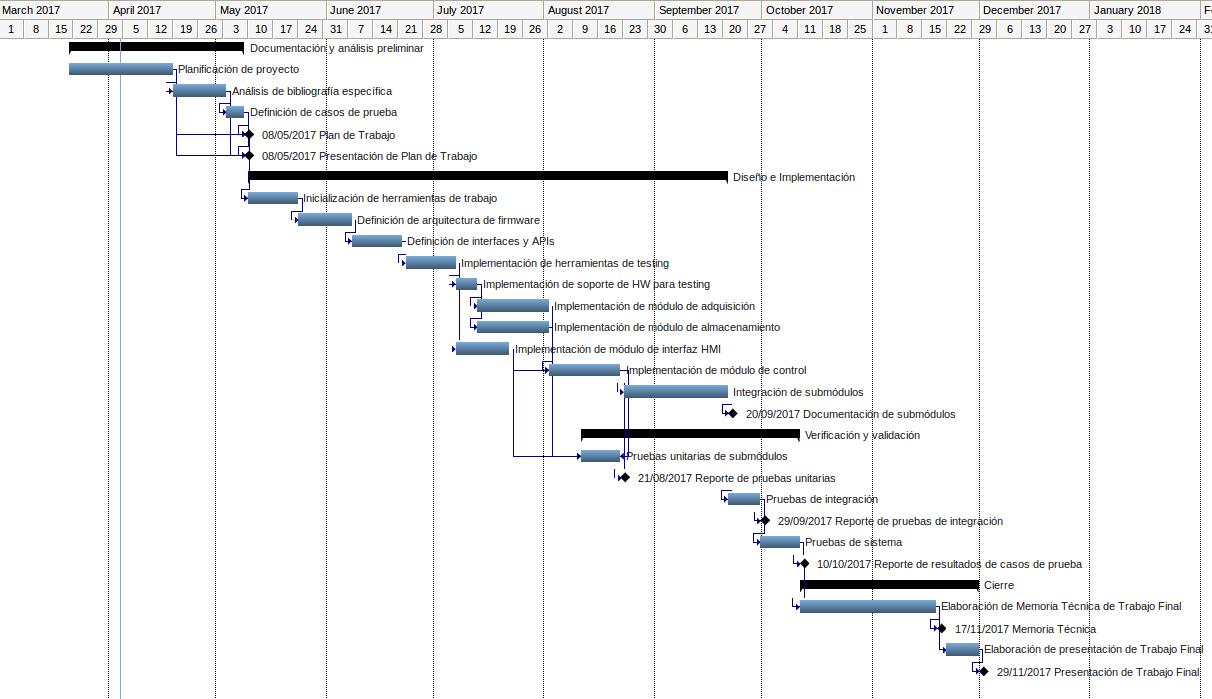
\includegraphics[height=.85\textheight]{./Figuras/Gantt-2.png}
\caption{Ejemplo de diagrama de Gantt rotado}
\label{fig:diagGantt}
\end{figure}

\end{landscape}

\end{consigna}


\section{12. Presupuesto detallado del proyecto}
\label{sec:presupuesto}

\begin{consigna}{red}
Si el proyecto es complejo entonces separarlo en partes:
\begin{itemize}
	\item Un total global, indicando el subtotal acumulado por cada una de las áreas.
	\item El desglose detallado del subtotal de cada una de las áreas.
\end{itemize}

IMPORTANTE: No olvidarse de considerar los COSTOS INDIRECTOS.

\end{consigna}

\begin{table}[htpb]
\centering
\begin{tabularx}{\linewidth}{@{}|X|c|r|r|@{}}
\hline
\rowcolor[HTML]{C0C0C0} 
\multicolumn{4}{|c|}{\cellcolor[HTML]{C0C0C0}COSTOS DIRECTOS} \\ \hline
\rowcolor[HTML]{C0C0C0} 
Descripción &
  \multicolumn{1}{c|}{\cellcolor[HTML]{C0C0C0}Cantidad} &
  \multicolumn{1}{c|}{\cellcolor[HTML]{C0C0C0}Valor unitario} &
  \multicolumn{1}{c|}{\cellcolor[HTML]{C0C0C0}Valor total} \\ \hline
 &
  \multicolumn{1}{c|}{} &
  \multicolumn{1}{c|}{} &
  \multicolumn{1}{c|}{} \\ \hline
 &
  \multicolumn{1}{c|}{} &
  \multicolumn{1}{c|}{} &
  \multicolumn{1}{c|}{} \\ \hline
\multicolumn{1}{|l|}{} &
   &
   &
   \\ \hline
\multicolumn{1}{|l|}{} &
   &
   &
   \\ \hline
\multicolumn{3}{|c|}{SUBTOTAL} &
  \multicolumn{1}{c|}{} \\ \hline
\rowcolor[HTML]{C0C0C0} 
\multicolumn{4}{|c|}{\cellcolor[HTML]{C0C0C0}COSTOS INDIRECTOS} \\ \hline
\rowcolor[HTML]{C0C0C0} 
Descripción &
  \multicolumn{1}{c|}{\cellcolor[HTML]{C0C0C0}Cantidad} &
  \multicolumn{1}{c|}{\cellcolor[HTML]{C0C0C0}Valor unitario} &
  \multicolumn{1}{c|}{\cellcolor[HTML]{C0C0C0}Valor total} \\ \hline
\multicolumn{1}{|l|}{} &
   &
   &
   \\ \hline
\multicolumn{1}{|l|}{} &
   &
   &
   \\ \hline
\multicolumn{1}{|l|}{} &
   &
   &
   \\ \hline
\multicolumn{3}{|c|}{SUBTOTAL} &
  \multicolumn{1}{c|}{} \\ \hline
\rowcolor[HTML]{C0C0C0}
\multicolumn{3}{|c|}{TOTAL} &
   \\ \hline
\end{tabularx}%
\end{table}


\section{13. Gestión de riesgos}
\label{sec:riesgos}

\begin{consigna}{red}
a) Identificación de los riesgos (al menos cinco) y estimación de sus consecuencias:
 
Riesgo 1: detallar el riesgo (riesgo es algo que si ocurre altera los planes previstos de forma negativa)
\begin{itemize}
	\item Severidad (S): mientras más severo, más alto es el número (usar números del 1 al 10).\\
	Justificar el motivo por el cual se asigna determinado número de severidad (S).
	\item Probabilidad de ocurrencia (O): mientras más probable, más alto es el número (usar del 1 al 10).\\
	Justificar el motivo por el cual se asigna determinado número de (O). 
\end{itemize}   

Riesgo 2:
\begin{itemize}
	\item Severidad (S): 
	\item Ocurrencia (O):
\end{itemize}

Riesgo 3:
\begin{itemize}
	\item Severidad (S): 
	\item Ocurrencia (O):
\end{itemize}


b) Tabla de gestión de riesgos:      (El RPN se calcula como RPN=SxO)

\begin{table}[htpb]
\centering
\begin{tabularx}{\linewidth}{@{}|X|c|c|c|c|c|c|@{}}
\hline
\rowcolor[HTML]{C0C0C0} 
Riesgo & S & O & RPN & S* & O* & RPN* \\ \hline
       &   &   &     &    &    &      \\ \hline
       &   &   &     &    &    &      \\ \hline
       &   &   &     &    &    &      \\ \hline
       &   &   &     &    &    &      \\ \hline
       &   &   &     &    &    &      \\ \hline
\end{tabularx}%
\end{table}

Criterio adoptado: 
Se tomarán medidas de mitigación en los riesgos cuyos números de RPN sean mayores a...

Nota: los valores marcados con (*) en la tabla corresponden luego de haber aplicado la mitigación.

c) Plan de mitigación de los riesgos que originalmente excedían el RPN máximo establecido:
 
Riesgo 1: plan de mitigación (si por el RPN fuera necesario elaborar un plan de mitigación).
  Nueva asignación de S y O, con su respectiva justificación:
  - Severidad (S): mientras más severo, más alto es el número (usar números del 1 al 10).
          Justificar el motivo por el cual se asigna determinado número de severidad (S).
  - Probabilidad de ocurrencia (O): mientras más probable, más alto es el número (usar del 1 al 10).
          Justificar el motivo por el cual se asigna determinado número de (O).

Riesgo 2: plan de mitigación (si por el RPN fuera necesario elaborar un plan de mitigación).
 
Riesgo 3: plan de mitigación (si por el RPN fuera necesario elaborar un plan de mitigación).

\end{consigna}


\section{14. Gestión de la calidad}
\label{sec:calidad}

\begin{consigna}{red}
Elija al menos diez requerientos que a su criterio sean los más importantes/críticos/que aportan más valor y para cada uno de ellos indique las acciones de verificación y validación que permitan asegurar su cumplimiento.

\begin{itemize} 
\item Req \#1: copiar acá el requerimiento.

\begin{itemize}
	\item Verificación para confirmar si se cumplió con lo requerido antes de mostrar el sistema al cliente. Detallar 
	\item Validación con el cliente para confirmar que está de acuerdo en que se cumplió con lo requerido. Detallar  
\end{itemize}

\end{itemize}

Tener en cuenta que en este contexto se pueden mencionar simulaciones, cálculos, revisión de hojas de datos, consulta con expertos, mediciones, etc.  Las acciones de verificación suelen considerar al entregable como ``caja blanca'', es decir se conoce en profundidad su funcionamiento interno.  En cambio, las acciones de validación suelen considerar al entregable como ``caja negra'', es decir, que no se conocen los detalles de su funcionamiento interno.

\end{consigna}

\section{15. Procesos de cierre}    
\label{sec:cierre}

\begin{consigna}{red}
Establecer las pautas de trabajo para realizar una reunión final de evaluación del proyecto, tal que contemple las siguientes actividades:

\begin{itemize}
	\item Pautas de trabajo que se seguirán para analizar si se respetó el Plan de Proyecto original:
	 - Indicar quién se ocupará de hacer esto y cuál será el procedimiento a aplicar. 
	\item Identificación de las técnicas y procedimientos útiles e inútiles que se emplearon, y los problemas que surgieron y cómo se solucionaron:
	 - Indicar quién se ocupará de hacer esto y cuál será el procedimiento para dejar registro.
	\item Indicar quién organizará el acto de agradecimiento a todos los interesados, y en especial al equipo de trabajo y colaboradores:
	  - Indicar esto y quién financiará los gastos correspondientes.
\end{itemize}

\end{consigna}


\end{document}
